\section{Our assigned user stories}
As described in \autoref{sprint-3-po-goals}, we had the goal of implementing the following three user stories.
\begin{itemize}\label{item:our-stories-sprint-3}
    \item Weekplanner\#133 - "As a guardian I would like to be able to logout when I'm on the choose citizen page so that I can return to the login page"
    \item Weekplanner\#92 - "As a developer I would like the application to use a default font so that I can easily change it"
    \item Weekplanner\#125 - "Exception thrown when rendering WeekPlanScreen, issue \#44"
\end{itemize}

\subsection{Weekplanner\#133}
The initial user story seemed simple to implement.
It just defined that the guardian should have the ability to logout when on the choose citizen page.
This evolved however after an initial pull request was created.
Based on feedback from the development groups and our workload, we decided to extend the issue to be the creation of a easily implementable navigation bar.
This navigation bar should have a default state, and allow for developers to include arguments defining which icons should be on the bar.

\begin{lstlisting}[caption={Building the appbar},label={lst:appbarbuild}]
  @override
  Widget build(BuildContext context) {
    toolbarBloc.updateIcons(appBarIcons, context);
    return AppBar(
        title: Text(title),
        backgroundColor: const Color(0xAAFF6600),
        actions: <Widget>[
          StreamBuilder<List<IconButton>>(
              initialData: const <IconButton>[],
              key: const Key('streambuilderVisibility'),
              stream: toolbarBloc.visibleButtons,
              builder: (BuildContext context, 
                AsyncSnapshot<List<IconButton>> snapshot) {
                return Row(
                  children: snapshot.data
                );
              }),
        ]);
  }
\end{lstlisting}
\autoref{lst:appbarbuild} shows the way we created the application bar widget.
We cleaned up the initial implementation of it, moving all the code related to instantiating icons to the \texttt{toolbar BLoC}.
\autoref{lst:appbarbuild} receives a context from which it updates the icons through the \texttt{updateIcons} method in the toolbar BLoc, which can be seen in \autoref{lst:updateicons}.
Within the \texttt{AppBar} widget that is returned, the icons are defined through the list of \texttt{IconButtons} on line 8.
\texttt{IconButton} is an enum we created defining all possible icons.
The order in which one inputs the arguments when instantiating the appbar determines in which order the icons are rendered on the page. 

\begin{lstlisting}[caption={Updating the icons in the appbar},label={lst:updateicons}]
  void updateIcons(List<AppBarIcon> icons, BuildContext context) {
  List<IconButton> _iconsToAdd;
  _iconsToAdd = <IconButton>[];

  if (icons == null) {
    icons = <AppBarIcon>[];
    icons.add(AppBarIcon.settings);
    icons.add(AppBarIcon.logout);
  }
  for (AppBarIcon icon in icons) {
    _addIconButton(_iconsToAdd, icon, context);
  }

  final BehaviorSubject<List<IconButton>> iconList =
      BehaviorSubject<List<IconButton>>.seeded(<IconButton>[]);
  iconList.add(_iconsToAdd);
  _visibleButtons = iconList;
}
\end{lstlisting}
\autoref{lst:updateicons} shows the method used in the \texttt{toolbarBloc}.
It takes a list of icons and a context as input.
It instantiates a list of the enum \texttt{IconButton}.
If the input list of icons is null, no arguments have been given to the appbar, meaning it should be created with the standard icons, settings and logout.
If any icons were defined, it uses the \texttt{\_addIconButton} method to add it.
Finally a new \texttt{BehaviorSubject} is created and the list of now instantiated buttons are added to it.
This is required for the appbar to update correctly whenever the icons that it is supposed to render changes.

\begin{lstlisting}[caption={Testing the appbar with certain icons},label={lst:appbaricontest}]
  testWidgets('Change to citizen button is displayed',
  (WidgetTester tester) async {
  final GirafAppBar girafAppBar = GirafAppBar(
    title: 'Ugeplan',
    appBarIcons: const <AppBarIcon>[AppBarIcon.changeToCitizen]);
  
  await tester.pumpWidget(makeTestableWidget(child: girafAppBar));
  await tester.pump();
  
  expect(find.byTooltip('Skift til borger tilstand'), findsOneWidget);
  });
  
\end{lstlisting}

\begin{figure}[h]
    \centering
    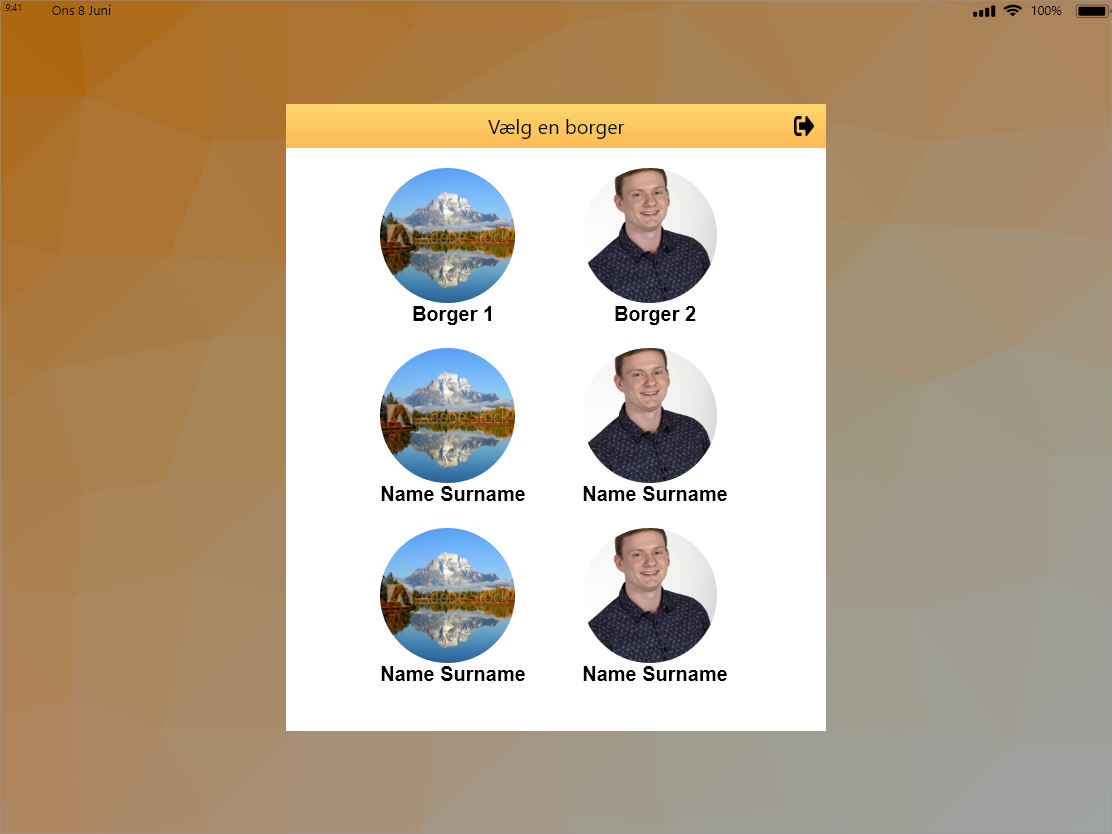
\includegraphics[width=1\textwidth]{sprint-3-133.png}
    \caption{The prototype for Weekplanner\#133}
    \label{fig:proto-weekplanner133}
  \end{figure}
\subsection{Weekplanner\#92}
This user story was relatively simple.
After discussing the issue of fonts with the customers, we were made aware that they wanted a font as close to text regularly written by humans as possible.
This required a change of font.
To make a new font the default used by the application, we added it to the theme settings when the application is initially run:

\begin{lstlisting}[caption={An excerpt of the run method},label={lst:fontfamily}]
  void _runApp() {
  runApp(MaterialApp(
      title: 'Weekplanner',
      theme: ThemeData(fontFamily: 'Quicksand'),
\end{lstlisting}
\autoref{lst:fontfamily} shows the beginning of the \texttt{\_runApp} method.
Changing the default font was done by adding the \texttt{fontFamily} to the theme.
The font family was defined in the \texttt{pubspec} file, which is where packages are specified in Flutter.
\begin{lstlisting}[caption={An excerpt of the pubspec file. Multiple assets are in the file for different styles, such as regular font.},label={lst:fontpubspec}]
  fonts:
  - family: 'Quicksand'
    fonts:
      - asset: assets/fonts/Quicksand-Bold.ttf
\end{lstlisting}
\subsection{Weekplanner\#125}
This issue related to the main screen of the weekplanner application.
Whenever it was opened, an exception would be thrown.
We deduced that it was related to the pictogram images. 
When the application would get these the exception would be thrown.
The issue turned out to be related to a custom widget called \texttt{PictogramImage}.
To change this, 


f,lexbox to set heiught or width, otherwise it defaults to 0 and blows up

Gesturedetector just lets the widget detect contact.

PiuctogramImage is a custom widget made by us.